\section{Implementation}
If implemented properly, the WLAN system will run as expected. All APs in the WLAN will update passwords simultaneously and regularly. Mobile devices get current passwords through an out-of-band channel and join WLAN. Once the WLAN password is updated, mobile devices have to update their own passwords in order to join WLAN again. If mobile devices can capture the beacon frame of the master AP and parse out the physical parameter, they can calculate out the new password and successfully join WLAN. If not, they cannot connect to the WLAN but can inform users to pass the physical access control and get into the specific location to get the physical parameter and calculate the new password. However, if the WLAN password have been updated for more than once, mobile devices can do nothing but inform users that they cannot join WLAN again. 

We have implemented a WLAN system deployed with the proposed evolving passwords mechanism and evaluated the influence of it. We have evaluated the following indexes. 

\subsection{Connection Delay of Mobile Devices)}
Connection delay of mobile devices means the time span from mobile devices receiving wireless signal to successfully joining WLAN. As mentioned above, mobile devices may use their own current passwords to join WLAN, or update their passwords and use new passwords to join WLAN. Also mobile devices may not be able to join WLAN as their own passwords are expired and unable to update. We have tested all of the above cases. We have also tested the connection delay of static passwords mechanism for comparison. Test results shows as below: 
\begin{table}
	\centering
	\caption{Test Results of Connection Delay of Mobile Devices}
	\label{Tab:4.1}
	\begin{tabularx}{\textwidth}{llll}
		\hline
		Static Passwords & Without Password Update & With Password Update & Unable to Join in \\
		\hline
		594.421ms & 600.694ms & 630.052ms & 0.091ms \\
		\hline
	\end{tabularx}
\end{table}
Test results show that password update has little influence on mobile devices connecting to WLAN. 

\subsection{Reconnection Delay of Mobile Devices)}
Reconnection delay of mobile devices means the time span from mobile devices losing connection of APs to reconnecting to APs. In our implementation, when getting new passwords, APs will restart to make new passwords come into force which means they will disconnect all mobile devices’ connections. Therefore, mobile devices need to reconnect to APs again. After restarting, APs will broadcast de-authenticate frames to all connected mobile devices. Then mobile devices will re-scan wireless signal. A separate program periodically query scanning results and parse serial numbers and physical parameters from scanning results. When it finds APs have updated their passwords and parses out new physical parameters, it will update mobile devices’ passwords and force mobile devices to reconnect to APs using new passwords. If mobile devices successfully reconnect to APs, the program will update mobile devices’ passwords. The reconnection delay is subject to query interval and shows as below: \begin{figure}
	\begin{center}
		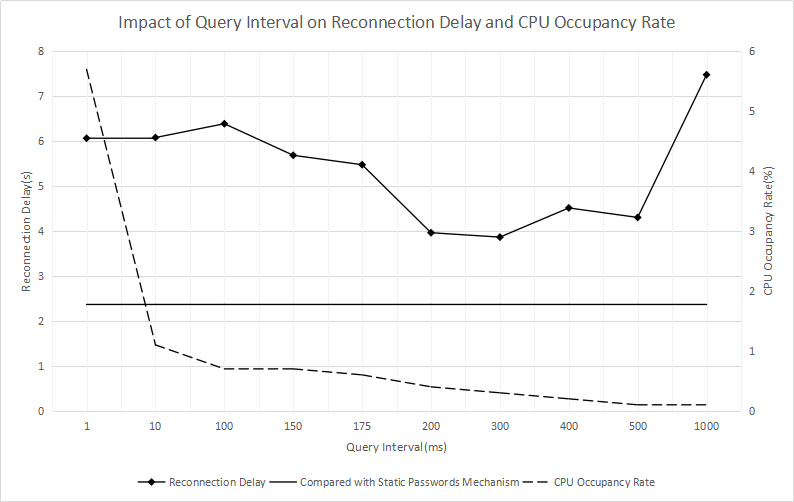
\includegraphics[width=\textwidth]{Results1.png}
		\caption{Impact of Query Interval on Reconnection Delay and CPU Occupancy Rate }
		\label{Fig:5.1}
	\end{center}
\end{figure}
According to our analysis, the bottleneck is re-scanning wireless signal. Scanning will last for about 1.5 seconds while it may happens for more than once. It should be noticed that there is almost no influence on memory occupation whatever the query interval is. 

\subsection{Update Delay of Slave APs}
Update delay of slave APs means the time gap between the master and slave APs update their own passwords separately. As mentioned above, the master AP update its passwords earlier than the slave APs. If the slave APs update their passwords much later than the master AP, it may cause problems on users when users move from wireless signal coverage of the master AP to wireless signal coverage of the slave APs. When users are under wireless signal coverage of the master AP and the master AP update its passwords, their mobile devices will update their passwords, too. However, when users move to the wireless signal coverage of the slave APs, they will be rejected to join WLAN because their mobile devices do not share the same password with the slave APs because the slave AP have not updated their passwords yet. It would be better if the update delay of slave APs can be as short as possible. If so, users can get a seamless experience when handover from one AP to another. When updating password, the slave APs request for a new password over and over again until a new password responded. The roll polling frequency influences the update delay of slave APs. A more frequent roll polling will shorten the update delay. However, it will also occupy a lot of system resources. We tested the influence of roll polling frequency. Test results shows as below: 
\begin{figure}
	\begin{center}
		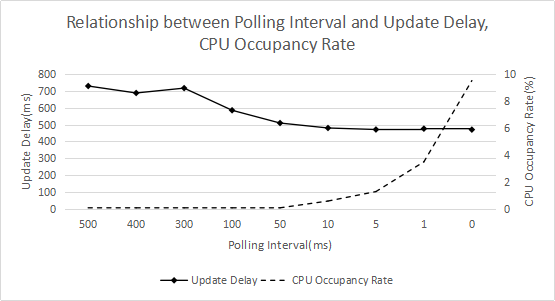
\includegraphics[width=\textwidth]{Results2.png}
		\caption{Relationship between Polling Interval and Update Delay, CPU Occupancy Rate}
		\label{Fig:5.2}
	\end{center}
\end{figure}
It should be noticed that there is almost no influence on memory occupation and network flow when requesting new passwords from the master AP whatever the roll polling frequency is. If set properly, all APs will update their own passwords in a short enough delay without occupying too much system resource. 
